% Editable report section: Performance Analysis and Results
\section{Performance Analysis and Results}
\label{sec:7}

Benchmarks used Windows 11 x64, Python 3.14.7 and an Intel64 Family 6 Model 165 processor. Each size used seed 2026 and the unit-square box. Table~\ref{tab:5} reports the median of three uninstrumented timing runs and separate memory measurements. Construction includes deduplication, normalization, the sweep, clipping and cell assembly; input generation, validation, plotting and export are excluded.

\begin{table}[!htbp]
\centering
\caption{Measured performance for seeded construction workloads.}
\label{tab:5}
\begin{tabularx}{\linewidth}{@{}rXXX@{}}
\toprule
\textbf{Sites} & \textbf{Median seconds} & \textbf{Python peak MiB} & \textbf{Process peak MiB} \\
\midrule
100 & 0.03294 & 0.70 & 23.67 \\
1,000 & 0.40641 & 7.38 & 41.42 \\
10,000 & 4.35665 & 65.08 & 217.48 \\
\bottomrule
\end{tabularx}
\end{table}

\begin{figure}[!htbp]
\centering
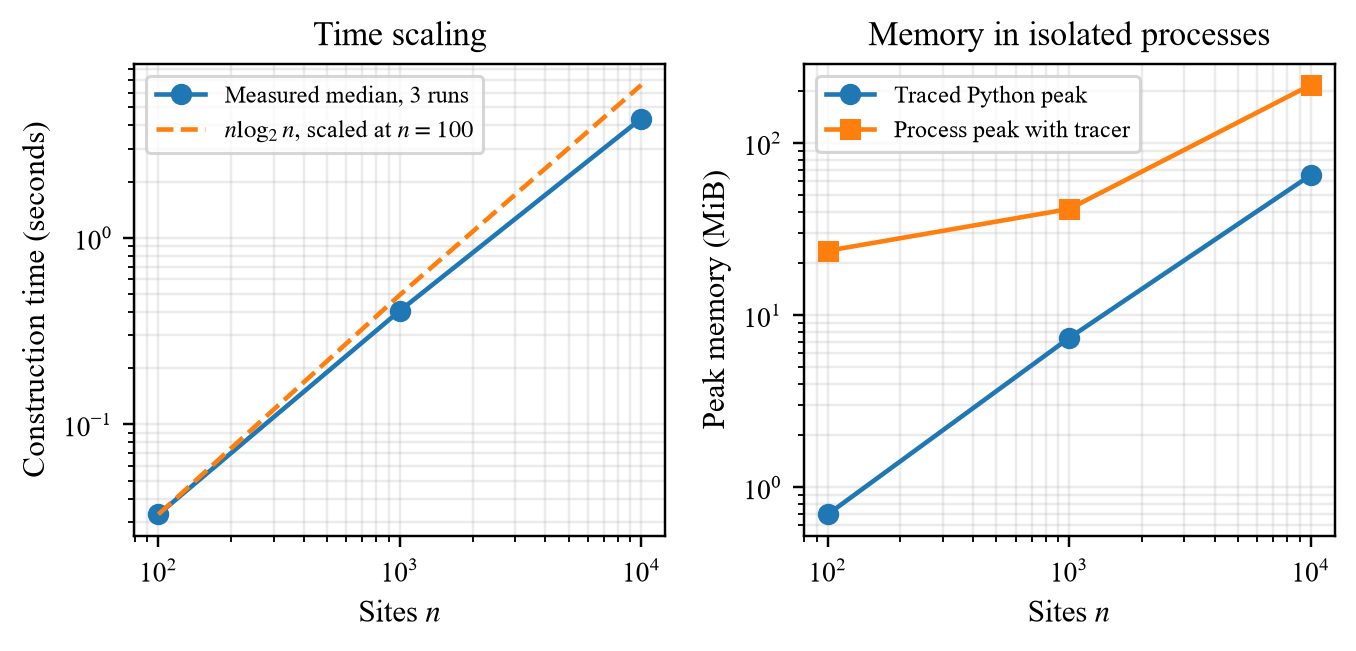
\includegraphics[width=1.0\linewidth,height=0.43\textheight,keepaspectratio]{scaling.png}
\caption{Measured construction time and isolated-process memory peaks.}
\label{fig:7}
\end{figure}

Memory was measured in fresh processes. Tracemalloc started after input generation and recorded Python allocations during construction. Process peak working set included the interpreter, input and instrumentation; it therefore does not measure uninstrumented incremental algorithmic memory \cite{pythontracemalloc}.

Tenfold input increases yielded time ratios of approximately 12.34 and 10.72. Python allocation peaks grew approximately tenfold. These observations are consistent with the intended \(O(n\log n)\) time and \(O(n)\) space, but three sizes do not prove asymptotic bounds. Full platform metadata, scope and per-run values are preserved in \path{results/benchmark.json}.
